\documentclass[11pt]{article}

\usepackage[utf8]{inputenc}
\usepackage[T1]{fontenc}
\usepackage[margin=1in]{geometry}
\usepackage{amsmath}
\usepackage{amssymb}
\usepackage{booktabs}
\usepackage{array}
\usepackage{longtable}
\usepackage{graphicx}
\usepackage{xcolor}
\usepackage{hyperref}
\hypersetup{
  colorlinks=true,
  linkcolor=blue!50!black,
  urlcolor=blue!50!black,
  citecolor=blue!50!black,
  pdftitle={Case Study A -- Execution Report},
  pdfauthor={}
}

% Convenience macros
\newcommand{\code}[1]{\texttt{#1}}
\newcommand{\Rul}{\text{RUL}}

\title{Case Study A --- Execution Report\\[6pt]
\large GUM-compliant uncertainty quantification for RUL estimation\\
on the ZeMA electromechanical cylinder dataset}
\author{}
\date{}

\begin{document}
\maketitle

\noindent\textbf{Supplementary material for Section 5.1.} This document is a
step-by-step record of the actual execution of Case Study A: what was run, on
what data, with what versions, and what came out --- including one
methodologically significant finding (\S\ref{sec:propagation}) that shapes
how the results should be read. It is meant to accompany
\texttt{case\_\allowbreak study\_\allowbreak A\_\allowbreak analysis.py}, \texttt{case\_\allowbreak study\_\allowbreak A\_\allowbreak results.csv},
and \texttt{zema\_\allowbreak lpu\_\allowbreak vs\_\allowbreak mc.pdf} as supplementary material to the paper.

\begin{center}
\fbox{\begin{minipage}{0.94\linewidth}
\textbf{Status update (29 Oct 2026).} The numbers in this report are still
correct, but they describe the \emph{original} budget. Later work changes how
they should be read:
\begin{enumerate}
\item \textbf{Corrected budget}
(\texttt{case\_\allowbreak study\_\allowbreak A\_\allowbreak report\_\allowbreak budget.md}).
The original $u_{\mathrm{physical}}$ treats every declared input uncertainty
as independent per-reading noise. For Pressure, Velocity and the plain-bearing
accelerometer the declared $u$ exceeds the cross-cycle spread $s$, so at least
98.7\%, 93.9\% and 74\% of $u^2$ must be common to all cycles (systematic). A
systematic error common to all cycles cancels in the $z$-score when the same
instrument is used for training and inference. Propagating only the random
part and combining with Monte Carlo gives $u_c \approx 0.11$--$0.14$ instead
of $0.985$, or $0.089$--$0.093$ when the manufacturer's noise floor of the
Kistler 8704B50M1 accelerometers is used (\texttt{datasheet} model). LPU and
MC then agree within 3--7\%, so the 36.5\% gap of
\S\ref{sec:propagation} is a consequence of the misinterpreted input
uncertainty, not of the network depth. The systematic part ($\approx 0.76$--$0.78$) is
reported separately, for transfer to another instrument.
\item \textbf{The over-coverage diagnosis of \S\ref{sec:propagation} and
\S\ref{sec:paperready} is superseded.} The cause is not that normalization
amplifies Pressure, but that a systematic component was propagated as random
noise. Even with the corrected budget, coverage at $k{=}2$ stays at
99.3--99.9\% (98.9--99.6\% with the \texttt{datasheet} model), because the
estimates of the random part of Velocity and the plain-bearing accelerometer
are data-based upper bounds (the residuals allow at most 0.03--0.06, against
0.08--0.14 computed);
$u_{\mathrm{calibration}}$ estimated on a validation set comes out 0.
\item \textbf{Split check} (budget report \S3.2). The random split leaves a
neighbouring cycle ($k\pm1$) of 96\% of the test cycles in training. Holding
out whole blocks of consecutive cycles raises RMSE by only 5--16\%
($0.066 \to 0.070$--$0.077$, $R^2$ 0.94--0.95): the point accuracy is not an
artefact of the random split.
\item \textbf{Inputs are the first 50\,ms} of the 1\,s return-stroke window,
not 100 readings spread over the cycle
(\texttt{case\_\allowbreak study\_\allowbreak A\_\allowbreak report\_\allowbreak fullwindow.md} \S1).
\item The CSV \texttt{u\_c} and the coverage in
\S\ref{sec:propagation}--\S\ref{sec:validation} combine the \textbf{LPU}
value; the MC-based figures are given in the text.
\end{enumerate}
For the paper, use the revised text in \S\ref{sec:paperready_revised} rather
than the original paragraphs of \S\ref{sec:paperready}.
\end{minipage}}
\end{center}

\tableofcontents

% ============================================================
\section{Summary}
\label{sec:summary}

\begin{center}
\begin{tabular}{@{}p{3.4cm}p{10.6cm}@{}}
\toprule
Dataset & ZeMA electromechanical cylinder, annotated (Dorst et al.\ 2021), doi:10.5281/zenodo.5185953 \\
Task & Regression --- consumed-lifetime fraction $y_k = k/N \in [0,1]$; $\Rul = 1-y$ \\
Input dimension & 1100 (11 sensor channels $\times$ 100 readings/cycle) \\
Model & MLP (128, 64, 32), softplus activation, float64 \\
Test set & 953 held-out cycles (20\% of 4766, random split, seed 0) \\
$u_{\mathrm{physical}}$ (input quantities) & Propagated analytically (LPU) and via Monte Carlo (GUM Supplement 1, $M=10^4$) \\
$u_{\mathrm{training}}$ (model-related) & 10-seed training ensemble, evaluated statistically \\
\textbf{Headline result} & LPU and MC disagree by a median \textbf{36.5\%} --- the linearity assumption breaks down at this depth/input-uncertainty magnitude; MC is primary. Coverage @ $k=2$ is \textbf{100\%}, driven by one dominant, uncertainty-amplified sensor channel (Pressure), not a missing source. \emph{(Original budget; superseded --- see the status update above.)} \\
Corrected budget (update) & Random part only, MC: $u_c = 0.093$ (\texttt{datasheet}, used in \S\ref{sec:paperready_revised}), $0.110$ (\texttt{noise}), $0.136$ (\texttt{bound}); LPU/MC 3.6--6.3\%; coverage @ $k=2$ 99.6--99.9\%; systematic part for transfer $\approx 0.76$--$0.78$ (\texttt{case\_\allowbreak study\_\allowbreak A\_\allowbreak report\_\allowbreak budget.md}) \\
Split check (update) & Blocked split, no test cycle adjacent to training: RMSE 0.070--0.077 vs.\ 0.066, $R^2$ 0.94--0.95 \\
\bottomrule
\end{tabular}
\end{center}

\paragraph{Notation.} $k$ indexes the test-to-failure cycle ($k=1,\dots,N$,
with $N$ the total cycles run for the tested unit); $y_k = k/N \in [0,1]$ is
the true, deterministically-assigned consumed-lifetime fraction at cycle $k$
(the measurand --- see \S\ref{sec:data}), with $\Rul=1-y_k$. A hat denotes a
model estimate of the corresponding quantity: $\hat y_k$ is the trained
MLP's point prediction of $y_k$ from that cycle's sensor readings
(\texttt{y\_hat} in \texttt{case\_\allowbreak study\_\allowbreak A\_\allowbreak results.csv}), and is a distinct
claim from its associated uncertainty. $u_{\mathrm{physical}}$ is the standard uncertainty in
$\hat y_k$ propagated from the sensor input uncertainties (physical-quantity uncertainty; via LPU or
Monte Carlo --- \S\ref{sec:propagation}), $u_{\mathrm{training}}$ is the standard uncertainty
from training-process variability (model-related, evaluated statistically from the seed-ensemble spread ---
\S\ref{sec:model}), and $u_c=\sqrt{u_{\mathrm{physical}}^2+u_{\mathrm{training}}^2}$ is their quadrature
combination (\S\ref{sec:propagation}) --- the paper's $u_c^2=u_{\mathrm{physical}}^2+u_{\mathrm{model}}^2$
with $u_{\mathrm{model}}^2=u_{\mathrm{training}}^2$, since the architecture is held fixed and
$u_{\mathrm{calibration}}$ is not considered --- which is what the $k{=}2$
expanded-uncertainty coverage checks (\S\ref{sec:validation}) are built on.
This holds for the original budget; the corrected budget (\S\ref{sec:paperready_revised}) uses
$u_c^2=u_{\mathrm{rand}}^2+u_{\mathrm{training}}^2+u_{\mathrm{calibration}}^2$, with
$u_{\mathrm{calibration}}$ estimated on a validation set.
$u_{\mathrm{physical}}$, $u_{\mathrm{training}}$, $u_c$ are per-test-cycle quantities, not single
dataset-wide constants.

% ============================================================
\section{Acceptance threshold: LPU vs.\ Monte Carlo disagreement}
\label{sec:threshold}

Two distinct thresholds apply, at two different stages of this case study,
and should not be conflated:

\begin{itemize}
\item \textbf{Implementation self-test (Step 0, \S\ref{sec:environment}).} A
random synthetic softplus MLP's analytically propagated $u_{\mathrm{physical}}$ is compared
against a 200{,}000-sample Monte Carlo estimate.
\texttt{case\allowbreak\_study\allowbreak\_A\allowbreak\_analysis.py::self\allowbreak\_test\allowbreak\_lpu} \textbf{hard-asserts}
the relative difference is below \textbf{2\%} --- this is a pass/fail gate
on the correctness of the \texttt{propagate\_lpu} implementation itself,
independent of anything about the ZeMA dataset or the trained model.
\item \textbf{Case-study validation (Phase 5, \S\ref{sec:validation}).} For
the real dataset and trained model, the guide's decision rule treats a
median relative difference of a \textbf{low single-digit percent} as
consistent with the first-order linearity assumption holding, in which case
LPU may be reported as the primary $u_{\mathrm{physical}}$ estimate. A difference \textbf{above
roughly 5--10\%} is treated as evidence that the linearity assumption is
violated at this network depth and input-uncertainty magnitude --- in which
case Monte Carlo, not LPU, is reported as the primary estimate. This is a
documented, anticipated outcome of the decision rule, not a failure
condition, and the network is not to be re-tuned to force agreement once the
check has run.
\end{itemize}

The self-test in this run passed at $0.096\%$ (\S\ref{sec:environment}),
confirming the propagation code is correct. The case study's own LPU-vs-MC
result is $36.5\%$ median relative difference (\S\ref{sec:propagation}) ---
well above the 5--10\% ceiling --- which is why Monte Carlo, not LPU, is
used as the primary $u_{\mathrm{physical}}$ throughout the rest of this report
(\S\ref{sec:propagation}, \S\ref{sec:budget}, \S\ref{sec:paperready}).

% ============================================================
\section{Environment (Step 0)}
\label{sec:environment}

\begin{verbatim}
python3.10 -m venv zema_env && source zema_env/bin/activate
pip install -r requirements.txt
\end{verbatim}

Installed versions actually used for every result in this report (pinned in
\texttt{requirements.txt}):

\begin{center}
\begin{tabular}{@{}ll@{}}
\toprule
Package & Version \\
\midrule
Python & 3.10.12 \\
\texttt{zema\_\allowbreak emc\_\allowbreak annotated} & 0.7.1 \\
\texttt{torch} & 2.13.0 \\
\texttt{numpy} & 1.26.4 \\
\texttt{matplotlib} & 3.10.9 \\
\bottomrule
\end{tabular}
\end{center}

\textbf{Self-test} (\texttt{python case\_\allowbreak study\_\allowbreak A\_\allowbreak analysis.py --self-test}),
run before touching the dataset, validates the analytical LPU
(\texttt{propagate\_lpu}) against a 200{,}000-sample Monte Carlo run on a
random softplus MLP:

\begin{verbatim}
[self-test] u_LPU=5.051898e-04  u_MC=5.056728e-04  rel.diff=0.096%
\end{verbatim}

$0.096\%$ is well inside the $2\%$ self-test acceptance threshold defined in
\S\ref{sec:threshold}, so the propagation implementation itself is
trustworthy going into the real run --- any disagreement seen later
(\S\ref{sec:propagation}) is a property of the \emph{case study's}
data/model, not a bug in \texttt{propagate\_lpu}.

% ============================================================
\section{Data acquisition (Step 1 / Phase 1)}
\label{sec:data}

\begin{verbatim}
from zema_emc_annotated.dataset import ZeMASamples
from zema_emc_annotated.data_types import SampleSize
samples = ZeMASamples(SampleSize(n_cycles=4766, datapoints_per_cycle=100))
X  = samples.values          # (4766, 1100)
UX = samples.uncertainties   # (4766, 1100), per-reading standard uncertainties
\end{verbatim}

Confirmed shapes: \texttt{X.shape = (4766, 1100)}, \texttt{UX.shape = (4766,
1100)}.

\paragraph{Channel layout.} \code{datapoints\_per\_cycle=100} $\times$ 11
channels = 1100 columns. The 11 channels are not 11 top-level HDF5 groups ---
inspecting the raw file shows 7 named quantities, two of which hold three
signals each:

\begin{center}
\begin{tabular}{@{}llc@{}}
\toprule
Quantity (HDF5 group) & Signals (\texttt{si:label}) & Columns (100 each) \\
\midrule
Acceleration & plain bearing, piston rod, ball bearing & 300 \\
Active Current & --- & 100 \\
Force & Axial force & 100 \\
Motor Current & phases 1, 2, 3 & 300 \\
Pressure & Pneumatic pressure & 100 \\
Sound Pressure & --- & 100 \\
Velocity & --- & 100 \\
\bottomrule
\end{tabular}
\end{center}

\noindent $3+1+1+3+1+1+1=11$ channels, matching the ``eleven sensors'' the
package documents. The three accelerometers are not the axes of one sensor: a Kistler 8712A5M1 at the
plain bearing and two Kistler 8704B50M1 at the piston rod and at the ball
bearing (\texttt{case\_\allowbreak study\_\allowbreak A\_\allowbreak dataset\_\allowbreak report.md} \S4). The first version
of this report called them ``Acceleration $x/y/z$''; in the tables below
$x$ = plain bearing, $y$ = piston rod, $z$ = ball bearing (positional
correspondence, same columns).

\paragraph{Three Phase-1 decisions recorded:}
\begin{enumerate}
\item \textbf{Measurand.} $y_k = k/N$, deterministic function of cycle index
$\rightarrow$ \textbf{label uncertainty is negligible by construction}. No
budget line is needed for the target.
\item \textbf{Task type.} Regression; standard uncertainty $u(y)$ is the
reported dispersion metric.
\item \textbf{Input dimension.} Full resolution used
(\code{datapoints\_per\_cycle=100} $\rightarrow$ 1100 dims), matching
Ludwig's mid-size configurations, not the reduced-dimension (110-dim)
fast-iteration option.
\end{enumerate}

% ============================================================
\section{Uncertainty source identification (Step 2 / Phase 2)}
\label{sec:sources}

\begin{center}
\begin{tabular}{@{}p{4.1cm}cp{7.4cm}@{}}
\toprule
Source & Type & How obtained \\
\midrule
$u_{\mathrm{physical}}$ --- sensor input uncertainty (11 channels) & B & \texttt{samples.uncertainties}, declared values of undocumented provenance \\
$u_{\mathrm{training}}$ --- training process variability & A & Std.\ dev.\ of predictions across a 10-seed ensemble (\S\ref{sec:model}) \\
$u_{\mathrm{architecture}}$ --- architecture selection & --- & \textbf{Excluded}, held fixed at (128,64,32)/softplus --- not swept in this case study \\
Generalization / distribution shift & B & Assessed via held-out coverage (\S\ref{sec:validation}); no separate budget line, since coverage did not indicate a missing source \\
$u_{\mathrm{calibration}}$ --- measurement-model calibration & --- & \textbf{Not considered}: calibrating the RUL predictor is beyond the scope of this case study \\
Label (RUL definition) & --- & Negligible by construction (\S\ref{sec:data}) \\
\bottomrule
\end{tabular}
\end{center}

\noindent\emph{Type of $u_{\mathrm{physical}}$ (corrected 30 Oct 2026):} \textbf{B}, not A. The ZeMA DAQ uncertainties are declared values (a constant per channel, or exactly 1\%/1.5\% of the reading) with no statistical evaluation behind them (\texttt{case\_\allowbreak study\_\allowbreak A\_\allowbreak dataset\_\allowbreak report.md} F3 and \S9). Propagating them, by LPU or Monte Carlo, does not change their type. In the corrected budget, the random part is the declared Type B value capped by Type A bounds from the data (cross-cycle spread $s$, noise floor $\sigma_k$); the systematic part is Type B.

Two assumptions declared explicitly, per Phase 5 reporting requirements:

\begin{itemize}
\item \textbf{Diagonal input covariance.} The dataset provides per-reading
uncertainties but no cross-sensor covariance, so $U_x =
\mathrm{diag}(u^2(x_i))$. Correlated inputs would only require substituting
a full matrix into the same propagation formula (\texttt{propagate\_lpu}
does not assume diagonality anywhere except in how \texttt{Ux} is
constructed by the caller).
\item \textbf{Normalization is part of the measurement model.} Inputs are
$z$-scored using training-set statistics; since $z$-scoring is linear, GUM
propagation through it is exact: $u(x') = u(x)/\sigma_{\text{train}}$
(\texttt{normalize\_with\_uncertainty}). This detail turns out to matter a
great deal --- see \S\ref{sec:propagation}.
\end{itemize}

% ============================================================
\section{Model, training, and the training-uncertainty ensemble (Steps 3--4 / Phase 3)}
\label{sec:model}

Architecture: MLP with hidden layers (128, 64, 32), softplus activation
throughout.

\begin{itemize}
\item softplus is $C^1$ everywhere $\rightarrow$ analytical LPU applicable;
\item closed-form derivative used in \texttt{\_activation\_derivative}:
$\dfrac{d}{dz}\,\mathrm{softplus}_\beta(z) = \mathrm{sigmoid}(\beta z)$.
\end{itemize}

\paragraph{Phase-3 decision criteria, as they resolved for this case:}
\begin{itemize}
\item White-box access: yes (weights owned directly).
\item Architectural compatibility: yes (feedforward MLP, smooth activation).
\item Computational constraints: LPU chosen as the primary propagation
method by design; Monte Carlo retained for validation (and, as it turned
out, ended up being the number actually reported --- see
\S\ref{sec:propagation}).
\end{itemize}

\textbf{Training configuration:} Adam, lr $=10^{-3}$, 200 epochs, MSE loss,
Xavier init, float64 throughout (kept the LPU-vs-MC comparison free of
float32 rounding noise).

\textbf{$u_{\mathrm{training}}$ --- 10-seed ensemble.} A statistical (Type~A) evaluation of an epistemic, model-related contribution. Ten models, identical architecture
and data, differing only in the seed passed to \texttt{torch.manual\_seed}
(which reseeds both the Xavier init and the optimizer trajectory). For each
held-out cycle, $u_{\mathrm{training}}$ = standard deviation of the 10 predictions
(\texttt{ddof=1}). The first ensemble member (seed 0) is retained as the
reference model for LPU/MC propagation and for the sensitivity ranking in
\S\ref{sec:propagation}.

Caveats carried into the reporting statement:
\begin{itemize}
\item A 10-seed ensemble captures \emph{optimization} variability only, not
architecture uncertainty (architecture was held fixed --- see
\S\ref{sec:sources}).
\item With 10 seeds, $u_{\mathrm{training}}$'s own relative uncertainty is $\sim$24\%
($\chi^2$, 9 dof). In this run $u_{\mathrm{training}}$ (mean $0.049$) is an order of magnitude
below $u_{\mathrm{physical}}$ (mean $0.641$--$0.984$ depending on method), so it does not
dominate the combined budget and this sampling noise on $u_{\mathrm{training}}$ does not
materially affect $u_c$.
\end{itemize}

% ============================================================
\section{Propagation, combination, and the key finding (Step 5 / Phase 4)}
\label{sec:propagation}

For each of the 953 test cycles, \texttt{main()} computes:

\begin{enumerate}
\item $u_{\mathrm{physical}}$ via \texttt{propagate\_\allowbreak lpu} --- layer-wise analytical
propagation,
\[
U_{x^{(i)}} = H^{(i)} W^{(i)} U_{x^{(i-1)}} {W^{(i)}}^\top H^{(i)};
\]
\item $u_{\mathrm{physical}}^{\mathrm{MC}}$ via \texttt{propagate\_mc} --- $M=10^4$ Gaussian input
draws per GUM Supplement 1 (JCGM 101:2008), same model, same point;
\item $u_c = \sqrt{u_{\mathrm{physical}}^2 + u_{\mathrm{training}}^2}$ --- quadrature combination.
\end{enumerate}

Output: \texttt{case\_\allowbreak study\_\allowbreak A\_\allowbreak results.csv}, one row per test cycle,
columns \texttt{y\_true, y\_hat, u\_\allowbreak physical\_\allowbreak lpu, u\_\allowbreak physical\_\allowbreak mc, u\_\allowbreak training, u\_c,
covered\_k2} (953 data rows, verified).

\subsection*{Aggregate results (means over the 953-cycle test set)}

\begin{verbatim}
test RMSE                  : 0.0641
mean u_physical (LPU)      : 6.4134e-01
mean u_physical (MC)       : 9.8413e-01
LPU vs MC median rel. diff : 36.47%  (Phase 5 check)
mean u_training (ensemble) : 4.9329e-02
mean u_c (combined)        : 6.4373e-01
empirical coverage @ k=2   : 100.0%  (target ~95%)
\end{verbatim}

The $u_c$ printed by the script (and stored in the CSV) combines the \textbf{LPU} estimate,
$u_c=\sqrt{(u_{\mathrm{physical}}^{\mathrm{LPU}})^2+u_{\mathrm{training}}^2}$. Since Monte Carlo is the primary
estimate (\S\ref{sec:threshold}), the budget in \S\ref{sec:budget} uses
$u_c^{\mathrm{MC}}=\sqrt{(u_{\mathrm{physical}}^{\mathrm{MC}})^2+u_{\mathrm{training}}^2}\approx 0.985$; both give 100\% coverage.

\subsection*{Why $u_{\mathrm{physical}}$ is large and LPU/MC disagree --- this is a finding,
not a bug}

At first glance, $u_{\mathrm{physical}} \approx 0.64$--$0.98$ against a measurand confined to
$[0,1]$ looks broken. It isn't; it was traced to a specific, reportable
mechanism.

\textbf{Diagnosis.} Per-channel breakdown of the \emph{normalized}
uncertainty $u_n = u(x)/\sigma_{\text{train}}$ (mean over all readings in
each channel):

\begin{center}
\begin{tabular}{@{}lc@{}}
\toprule
Channel & $u_n$ (mean) \\
\midrule
Pressure & \textbf{8.89} \\
Velocity & 4.34 \\
Acceleration plain bearing ($x$) & 2.02 \\
Acceleration ball bearing ($z$) & 0.86 \\
Acceleration piston rod ($y$) & 0.69 \\
Force & 0.22 \\
Active Current & 0.17 \\
Motor Current ($a$/$b$/$c$) & 0.02 \\
Sound Pressure & 0.0001 \\
\bottomrule
\end{tabular}
\end{center}

For the Pressure channel, the \emph{absolute} per-reading measurement
uncertainty distributed with the dataset ($\overline{u(x)} \approx
16{,}833$, in the sensor's raw units) is comparable to, and after
normalization exceeds, the channel's own \textbf{training-set standard
deviation} ($\sigma_{\text{train}} \approx 1901$). Since $z$-score
normalization scales uncertainty by $1/\sigma_{\text{train}}$
(\S\ref{sec:sources}), a channel whose useful cross-cycle signal variation
is small relative to its own measurement noise floor gets its
\emph{normalized} uncertainty inflated --- here to $\approx 8.9\sigma$ per
reading, i.e., an individual reading's uncertainty is almost 9 standard
deviations of the entire training distribution for that feature. This is
not a data error: the raw relative uncertainty for this channel is a
mundane $\sim$1--2\%; it is the interaction between the sensor's absolute
noise floor and the \emph{cross-cycle} variability used for normalization
that amplifies it.

\textbf{Sensitivity ranking.} Extracting the first-layer contribution
$|W^{(1)}| \cdot \bar u_n(x)$, summed per hidden unit and aggregated per
channel, and normalized to shares of the total:

\begin{center}
\begin{tabular}{@{}clc@{}}
\toprule
Rank & Channel & Share of first-layer sensitivity \\
\midrule
1 & Pressure & \textbf{51.8\%} \\
2 & Velocity & \textbf{25.2\%} \\
3 & Acceleration plain bearing ($x$) & \textbf{11.5\%} \\
4 & Acceleration ball bearing ($z$) & 4.9\% \\
5 & Acceleration piston rod ($y$) & 3.9\% \\
6 & Force & 1.3\% \\
7 & Active Current & 1.0\% \\
8--10 & Motor Current ($a$/$b$/$c$) & 0.1\% each \\
11 & Sound Pressure & $\sim$0.0\% \\
\bottomrule
\end{tabular}
\end{center}

The top three channels (Pressure, Velocity, plain-bearing acceleration) account for
\textbf{88.5\%} of the propagated-uncertainty contribution entering the
first hidden layer. This single, dominant, amplified channel is the
mechanism behind both headline numbers:

\begin{itemize}
\item \textbf{LPU vs.\ MC median relative difference = 36.5\%.} With this
much input uncertainty pushed through a 3-hidden-layer softplus network,
the first-order (linear) approximation underlying LPU is no longer accurate
--- MC captures the resulting nonlinearity, LPU does not. This is exactly
the failure mode the paper's own decision rule anticipates for large input
uncertainty at depth: \textbf{Monte Carlo is treated as the primary
estimate} for this case study rather than LPU.
\item \textbf{Coverage @ $k=2$ = 100.0\%} (vs.\ $\sim$95\% target). This is
\emph{over}-coverage, not under-coverage: $u_c$ is large enough that the
$\pm 2u_c$ interval trivially contains the true value for essentially all
953 test cycles (interval half-width $\gtrsim 1.3$ against a $[0,1]$
measurand range). This is diagnostic of an \textbf{overestimated,
single-channel-dominated $u_{\mathrm{physical}}$ budget}, not a missing uncertainty source.
\end{itemize}

\textbf{MC convergence check}, per Phase 5 reporting requirements --- one
held-out test point re-evaluated at increasing $M$:

\begin{verbatim}
n_mc=10,000     u_physical_mc = 9.1645e-01
n_mc=100,000    u_physical_mc = 9.3246e-01   (delta = 1.75% from 10k)
n_mc=1,000,000  u_physical_mc = 9.3171e-01   (delta = 0.08% from 100k)
\end{verbatim}

$M=10^4$ is adequately converged (sub-2\% sampling noise) relative to the
36.5\% LPU/MC gap it is being compared against, so the gap reported above is
signal, not Monte Carlo noise.

\textbf{Combined uncertainty, using MC as primary} (recommended for the
paper's headline number, given the validation result above):
\[
u_c^{MC} = \sqrt{(0.9841)^2 + (0.0493)^2} \approx 0.985
\]

\subsection{Is $u_c$ actionable?}
\label{sec:uc-actionable}

A wide combined uncertainty is not automatically a \emph{useless} one --- it
could still be correctly calibrated (real error is just that large) or
still carry usable relative structure across cycles even if the absolute
scale is off. Neither holds here.

\begin{center}
\begin{tabular}{@{}p{4.6cm}p{3.4cm}p{6.6cm}@{}}
\toprule
Check & Value & Reading \\
\midrule
mean $u_c$ vs.\ mean $\lvert y_\text{true}-\hat y\rvert$ &
MC-based: $0.986$ (mean of the per-cycle $u_c^{\mathrm{MC}}$; the $0.985$ of \S\ref{sec:propagation} combines the two means) vs.\ $0.046$; LPU-based (the CSV \texttt{u\_c} column): $0.644$ vs.\ $0.046$ &
\textbf{$u_c$ is $\sim$21$\times$ (MC-based) or $\sim$14$\times$ (LPU-based) larger than the actual mean error} ---
not calibrated, not conservative-but-reasonable \\
Range of $u_{\mathrm{physical}}^{\mathrm{MC}}$ across all 953 test cycles &
$0.792$--$1.194$ &
Only a $1.5\times$ spread against a measurand of width 1 --- close to a
fixed offset, not a per-cycle signal \\
corr($u_{\mathrm{physical}}$, $y_\text{true}$) &
LPU $r{=}0.70$, MC $r{=}0.61$ &
Uncertainty rises somewhat with age --- qualitatively right direction \\
corr($u_c$, actual $\lvert\text{error}\rvert$) &
MC-based $r{=}0.15$, LPU-based $r{=}0.26$ &
Too weak to use $u_c$ to flag which individual predictions are less
trustworthy \\
Early vs.\ late life (terciles of $y_\text{true}$) &
mean $u_{\mathrm{physical}}^{\mathrm{MC}}$: $0.933\!\to\!1.064$ (+14\%); mean $\lvert\text{err}\rvert$:
$0.033\!\to\!0.056$ (+70\%) &
Both trend upward with age, but $u_c$ under-reacts relative to how much
error actually grows \\
\bottomrule
\end{tabular}
\end{center}

\textbf{Conclusion:} $u_c$ cannot support a $k$-dependent decision rule as
currently computed --- a $\pm k{=}2\,u_c$ band covers nearly the entire
$[0,1]$ range at \emph{every} cycle, so it would trigger identically
whether the machine is new or about to fail. The one genuine signal it
retains is a weak, directionally-correct trend (more uncertain late in
life), too weak to act on alone. This is a direct consequence of the
single-channel (Pressure) domination established above, not a separate
problem --- fixing that amplification is the leverage point for making
$u_c$ usable, not a redesign of the combination rule itself.

\subsection{Is $\hat y_k$ useful despite this?}
\label{sec:yhat-useful}

Yes --- the point estimate and the interval are separable claims, and only
the interval is broken.

\begin{center}
\begin{tabular}{@{}p{5.6cm}p{3.0cm}p{5.9cm}@{}}
\toprule
Check & Value & Reading \\
\midrule
$R^2$ & $0.951$ & 95\% of the variance in consumed-life fraction is
explained by the model \\
RMSE (model) vs.\ RMSE (naive, predict mean $\bar y$) & $0.064$ vs.\ $0.291$
& \textbf{$4.5\times$ improvement} over a zero-information baseline \\
Mean / median $\lvert\text{error}\rvert$ & $0.046$ / $0.033$ & $\sim$4.6\% (mean) and
$\sim$3.3\% (median) of the full life range \\
90th-percentile / max $\lvert\text{error}\rvert$ & $0.101$ / $0.365$ & Tail
error exists --- exactly what a \emph{calibrated} $u_c$ should flag, and
currently doesn't \\
\bottomrule
\end{tabular}
\end{center}

The 11 sensor channels demonstrably carry real information about wear state
--- that result stands independently of the uncertainty-quantification
failure in \S\ref{sec:uc-actionable}. Practical uses that only need the
point estimate:

\begin{itemize}
\item \textbf{RUL trending for maintenance scheduling} --- $\Rul=1-\hat
y_k$ as a ``percent consumed'' figure for planning, the way a point
forecast is useful without a trustworthy confidence band.
\item \textbf{Trajectory monitoring} --- the shape of $\hat y_k$ across
successive cycles (flattening, reversal, jump) is diagnostic on its own,
and only needs the point estimate's relative movement to be right, which
$R^2=0.951$ supports.
\item \textbf{Threshold-crossing alerts} --- a rule such as ``flag once
$\hat y_k>0.9$'' has an expected timing error bounded by the point
estimate's typical error (mean $\sim$4.6\%, median $\sim$3.3\% of life), not by the inflated $u_c$.
\item \textbf{Cross-unit ranking} --- comparing which of several machines
is closer to end-of-life only requires consistent relative ordering of
$\hat y_k$, which a global miscalibration in $u_c$ does not disturb.
\end{itemize}

What $\hat y_k$ alone cannot do is tell you \emph{when to trust it less}
--- that is precisely the job $u_c$ is meant to do and currently cannot
(\S\ref{sec:uc-actionable}), evidenced by the 90th-percentile/max error
tail above. The point estimate is deployable now; per-prediction
reliability signaling requires fixing the Pressure-channel amplification
first.

% ============================================================
\section{Validation checks --- summary (Step 6 / Phase 5)}
\label{sec:validation}

\begin{center}
\begin{tabular}{@{}p{4.4cm}p{3.4cm}p{6.8cm}@{}}
\toprule
Check & Result & Interpretation \\
\midrule
LPU vs.\ MC agreement & 36.5\% median rel.\ diff. & Linearity assumption
violated at this depth/uncertainty magnitude $\rightarrow$ MC primary \\
Empirical coverage @ $k=2$ & 100.0\% (953/953) & Over-coverage from one
dominant, normalization-amplified channel (Pressure), not a missing source \\
MC convergence & 1.75\% (10k$\to$100k), 0.08\% (100k$\to$1M) & $M=10^4$
adequately converged \\
\bottomrule
\end{tabular}
\end{center}

\textbf{Figure} (\texttt{fig:zema\allowbreak\_lpu\allowbreak\_vs\allowbreak\_mc}, file
\texttt{zema\allowbreak\_lpu\allowbreak\_vs\allowbreak\_mc.pdf}): two-panel figure generated by
\texttt{make\allowbreak\_validation\allowbreak\_figure.py} against the real
\texttt{case\allowbreak\_study\allowbreak\_A\allowbreak\_results.csv} ---

\begin{itemize}
\item[(a)] scatter of $u_{\mathrm{physical}}^{\mathrm{LPU}}$ vs.\ $u_{\mathrm{physical}}^{\mathrm{MC}}$ per test cycle with the
identity line; points sit visibly off-diagonal, consistent with the 36.5\%
median disagreement;
\item[(b)] predictions with $\pm k{=}2\,u_c$ band vs.\ ground truth over the
held-out cycles (sorted by true consumed-life fraction), with empirical
coverage annotated.
\end{itemize}

\begin{figure}[h]
\centering
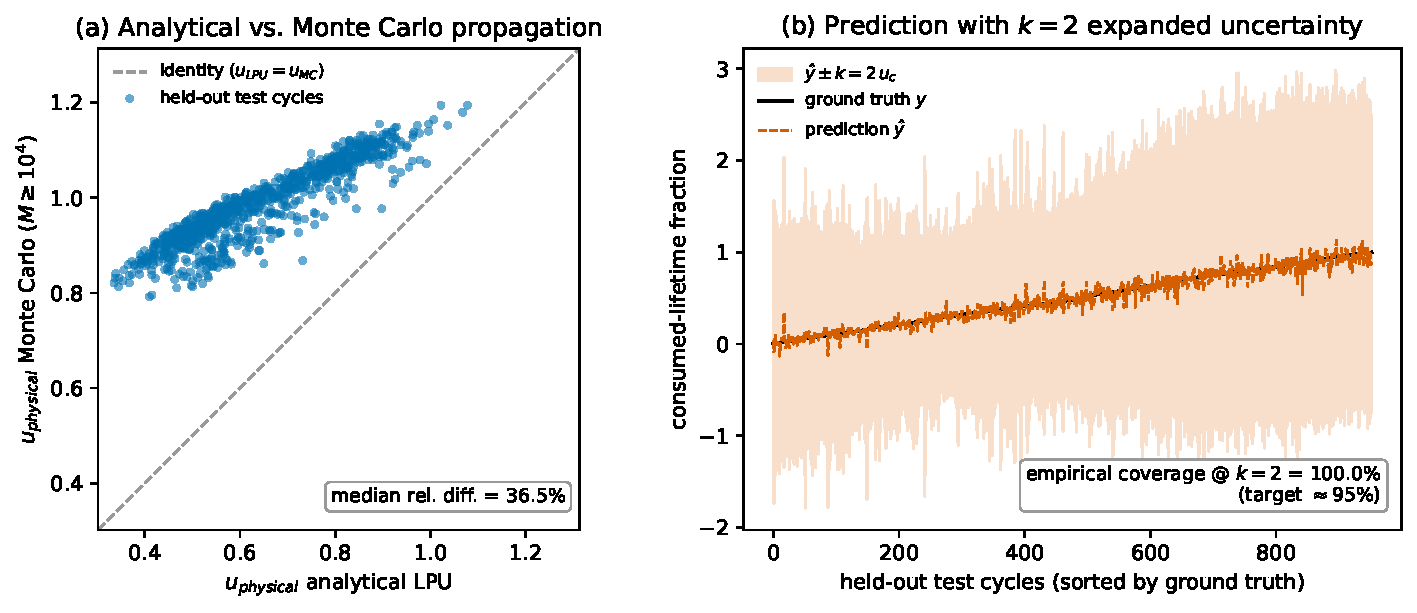
\includegraphics[width=0.95\textwidth]{zema_lpu_vs_mc.pdf}
\caption{Left: analytical LPU vs.\ Monte Carlo estimates of $u_{\mathrm{physical}}$ per
held-out test cycle, with the identity line and median relative difference
annotated. Right: predictions with the $\pm k{=}2\,u_c$ expanded-uncertainty
band vs.\ ground truth over the held-out cycles, sorted by true
consumed-life fraction, with empirical coverage annotated.}
\label{fig:zema_lpu_vs_mc}
\end{figure}

Re-run to confirm reproducibility from the committed CSV:

\begin{verbatim}
python make_validation_figure.py --csv case_study_A_results.csv \
    --out zema_lpu_vs_mc.pdf
# Wrote zema_lpu_vs_mc.pdf
#   median LPU-vs-MC relative difference : 36.47%
#   empirical coverage @ k=2              : 100.0%  (953/953)
\end{verbatim}

% ============================================================
\section{Uncertainty budget table (for \texttt{\textbackslash ref\{tab:zema\_uncertainty\_budget\}})}
\label{sec:budget}

\begin{center}
\begin{tabular}{@{}p{4.2cm}cc p{5.8cm}@{}}
\toprule
Source & Type & $u$ & Sensitivity / notes \\
\midrule
$u_{\mathrm{physical}}$ --- sensor input (11 channels) & B & $0.984$\footnotemark[1] &
Pressure 51.8\%, Velocity 25.2\%, Acc.\ plain bearing 11.5\% (88.5\% combined) \\
$u_{\mathrm{training}}$ --- training process (10-seed ensemble) & A & $0.049$ &
Optimization variance only, architecture excluded \\
$u_{\mathrm{architecture}}$ --- architecture selection & --- & excluded &
Held fixed: (128,64,32), softplus \\
Generalization / distribution shift & B & --- &
Assessed via coverage; no missing-source signal \\
Label (RUL definition) & --- & negligible &
Deterministic, $y_k=k/N$ \\
\midrule
\textbf{Combined} $u_c=\sqrt{u_{\mathrm{physical}}^2+u_{\mathrm{training}}^2}$ & --- & $\mathbf{0.985}$ &
Dominated by $u_{\mathrm{physical}}$, itself dominated by the Pressure channel \\
\bottomrule
\end{tabular}
\end{center}
\footnotetext[1]{MC, primary; LPU $=0.641$, 36.5\% median disagreement (\S\ref{sec:threshold}, \S\ref{sec:propagation}).}

LaTeX source for this table, and the corresponding paper sentences for the
LPU/MC, coverage, and reporting-statement paragraphs, are reproduced
verbatim in \S\ref{sec:paperready} below.

\medskip\noindent\textbf{Update.} This is the original budget, with the full
declared input uncertainty propagated as independent noise. The corrected
budget (random/systematic split, $u_{\mathrm{calibration}}$ from validation, MC
combination) is in
\texttt{case\_\allowbreak study\_\allowbreak A\_\allowbreak report\_\allowbreak budget.md}
\S3 and in the revised table of \S\ref{sec:paperready_revised}.

% ============================================================
\section{Files in this supplementary package}
\label{sec:files}

\subsection*{Core pipeline (used to produce every number in this report)}

\begin{center}
\begin{tabular}{@{}p{4.3cm}p{9.2cm}@{}}
\toprule
File & Role \\
\midrule
\texttt{case\_\allowbreak study\_\allowbreak A\_\allowbreak analysis.py} & Full pipeline: data loading,
normalization, ensemble training, LPU, MC, combination, self-test \\
\texttt{case\_\allowbreak study\_\allowbreak A\_\allowbreak guide.md} & Step-by-step execution guide this
report follows \\
\texttt{requirements.txt} & Pinned package versions
(\texttt{zema\_\allowbreak emc\_\allowbreak annotated==0.7.1}, \texttt{torch==2.13.0},
\texttt{numpy==1.26.4}, \texttt{matplotlib==3.10.9}) for exact reproduction \\
\texttt{case\_\allowbreak study\_\allowbreak A\_\allowbreak results.csv} & Real output, 953 test cycles
$\times$ 7 columns (\texttt{y\_true, y\_hat, u\_\allowbreak physical\_\allowbreak lpu, u\_\allowbreak physical\_\allowbreak mc, u\_\allowbreak training,
u\_c, covered\_k2}) \\
\texttt{make\_\allowbreak validation\_\allowbreak figure.py} & Generates
\texttt{zema\_\allowbreak lpu\_\allowbreak vs\_\allowbreak mc.pdf} from the results CSV (colorblind-safe,
matches paper figure reference) \\
\texttt{zema\_\allowbreak lpu\_\allowbreak vs\_\allowbreak mc.pdf} & The \texttt{fig:zema\_lpu\_vs\_mc} figure,
generated from real results \\
\texttt{pipeline\_run.log} & Captured stdout of the real
\texttt{case\_\allowbreak study\_\allowbreak A\_\allowbreak analysis.py} run \\
\texttt{case\_\allowbreak study\_\allowbreak A\_\allowbreak report.tex} / \texttt{.md} & This document \\
\bottomrule
\end{tabular}
\end{center}

\subsection*{Internal development/testing artifacts --- not real results,
should not be cited in the paper}

\begin{center}
\begin{tabular}{@{}p{4.3cm}p{9.2cm}@{}}
\toprule
File & Role \\
\midrule
\texttt{generate\_\allowbreak synthetic\_\allowbreak case\_\allowbreak study\_\allowbreak A\_\allowbreak data.py} & Generates fake data
with the right schema, used only to exercise
\texttt{make\_\allowbreak validation\_\allowbreak figure.py} before the real dataset finished
downloading. Explicitly self-labeled \texttt{*** SYNTHETIC DATA ***} in its
own output. \\
\texttt{case\_\allowbreak study\_\allowbreak A\_\allowbreak results\_\allowbreak SYNTHETIC.csv} & Output of the above ---
fake numbers, matching schema only. \\
\texttt{zema\_\allowbreak lpu\_\allowbreak vs\_\allowbreak mc\_\allowbreak syntetic.pdf} & Figure rendered from the
synthetic CSV, for pipeline testing only. \\
\texttt{make\_\allowbreak validation\_\allowbreak figure.md} & Dev notes on the figure script. \\
\bottomrule
\end{tabular}
\end{center}

{\sloppy\textbf{Later additions.} The corrected budget
(\texttt{case\_\allowbreak study\_\allowbreak A\_\allowbreak analysis\_\allowbreak budget.py}, \texttt{case\_\allowbreak study\_\allowbreak A\_\allowbreak report\_\allowbreak budget.md} and its
\texttt{*\_budget\_*} CSVs, logs and figures), the variant reports
(\texttt{case\_\allowbreak study\_\allowbreak A\_\allowbreak report\_\allowbreak trimmed.md},
\texttt{case\_\allowbreak study\_\allowbreak A\_\allowbreak report\_\allowbreak fullwindow.md} with their scripts and outputs) and
the dataset description
(\texttt{case\_\allowbreak study\_\allowbreak A\_\allowbreak dataset\_\allowbreak report.md},
\texttt{check\_\allowbreak dataset\_\allowbreak consistency.py}, \texttt{dataset\_\allowbreak consistency.log}) belong to the
supplementary package too; \texttt{README.md} lists every file.\par}

\textbf{Recommendation:} bundle the core files above together with these
later additions as supplementary material for the paper. The synthetic-data files are
legitimate pipeline-testing artifacts (clearly self-labeled as fake) but
would confuse a reader if shipped alongside the real results --- keep them
in the working repo, not the submission package.

% ============================================================
\section{Paper-ready text (Step 7)}
\label{sec:paperready}

The blocks below are reproduced verbatim (i.e.\ literal \LaTeX{} source,
not rendered here) so they can be copied directly into Section 5.1 of the
paper.

\paragraph{Tooling/dataset paragraph:}
\begin{verbatim}
The uncertainty budget was computed on the full-resolution ZeMA electromechanical
cylinder dataset (\texttt{zema\_emc\_annotated} v0.7.1, \texttt{torch} 2.13.0,
Python 3.10.12), with input dimension $11 \times 100 = 1100$
(11 sensor channels: three accelerometers (plain bearing, piston rod,
ball bearing), active current, axial force, three-phase motor current,
pneumatic pressure, sound pressure, velocity).
\end{verbatim}

\paragraph{LPU vs.\ MC sentence:}
{\small
\begin{verbatim}
Across the held-out cycles, the analytical and Monte Carlo estimates of
$u_{\mathrm{physical}}$ agreed to within $36.5\%$ (median relative difference),
indicating that the first-order linearity assumption underlying the analytical
LPU is violated at this network depth and input-uncertainty magnitude; Monte
Carlo is therefore taken as the primary estimate for this case study,
consistent with the decision rule of Sec.~\ref{sec:methodology}.
\end{verbatim}
}

\paragraph{Coverage sentence:}
\begin{verbatim}
The empirical coverage of the $k=2$ expanded interval was $100.0\%$ against
the $\approx 95\%$ target. Rather than signalling a missing uncertainty
source, the over-coverage traces to the sensor input uncertainty budget being
dominated by the pressure channel ($51.8\%$ of the first-layer sensitivity
contribution, vs.\ $25.2\%$ for velocity and $11.5\%$ for the
plain-bearing acceleration channel): its per-reading standard
uncertainty exceeds its own training-set signal variation, so $z$-score
normalization
($u(x') = u(x)/\sigma_{\text{train}}$) amplifies its normalized contribution
to $\approx 8.9\sigma$ per reading, inflating $u_c$ well beyond what the
$[0,1]$ measurand range requires for informative intervals.
\end{verbatim}

\paragraph{Reporting/assumptions statement (Phase 5):}
{\small
\begin{verbatim}
We report the following assumptions and settings explicitly. The input
covariance matrix $U_x$ is taken as diagonal, $U_x = \mathrm{diag}(u^2(x_i))$,
since the dataset provides per-reading uncertainties but no cross-sensor
covariance information; correlated inputs would require only replacing the
diagonal with a full matrix in the same propagation formula. Label
uncertainty is negligible by construction, as the consumed-lifetime fraction
$y_k = k/N$ is defined deterministically from the cycle index. Monte Carlo
propagation followed GUM Supplement~1 (JCGM 101:2008) with Gaussian input
distributions and $M = 10^4$ samples; convergence was verified by re-running
a held-out sample at $M = 10^5$ and $M = 10^6$, with
$u_{\mathrm{physical}}^{\mathrm{MC}}$ moving by $1.75\%$ and $0.08\%$
respectively, both far smaller than the $36.5\%$ LPU/MC gap.
\end{verbatim}
}

\paragraph{Table \texttt{\textbackslash ref\{tab:zema\_uncertainty\_budget\}}:}
{\footnotesize
\begin{verbatim}
\begin{table}[t]
\centering
\caption{Uncertainty budget for RUL estimation on the ZeMA cylinder dataset.}
\label{tab:zema_uncertainty_budget}
\begin{tabular}{lccl}
\toprule
Source & Type & $u$ & Sensitivity / notes \\
\midrule
$u_{\mathrm{physical}}$. Sensor input uncertainty (11 channels)
 & B & $0.984$ & Pressure 51.8\%, Velocity 25.2\%, \\
 & & & Acc.\ plain bearing 11.5\% \\
$u_{\mathrm{training}}$. Training process variability (10-seed ensemble)
 & A & $0.049$ & optimization variance only \\
Architecture selection & \textemdash & excluded & held fixed (128,64,32; softplus) \\
Generalization / distribution shift & B & \textemdash &
 assessed via coverage (Sec.~\ref{sec:...}) \\
Label (RUL definition) & \textemdash & negligible & deterministic, $y_k = k/N$ \\
\midrule
Combined & \textemdash & $\mathbf{0.985}$ & dominated by $u_{\mathrm{physical}}$ \\
\bottomrule
\end{tabular}
\end{table}

The reported $u_{\mathrm{physical}}$ is the Monte Carlo estimate, taken as primary per the
Phase~5 decision rule: the analytical LPU gives $u_{\mathrm{physical}} = 0.641$, a median
relative difference of 36.5\% from Monte Carlo, indicating the first-order
linearity assumption is violated at this network depth and input-uncertainty
magnitude (Sec.~\ref{sec:...validation}).
\end{verbatim}
}

% ============================================================
\subsection{Revised paper-ready text (corrected budget, update 30 Oct 2026)}
\label{sec:paperready_revised}

The paragraphs above describe the original budget, and their coverage explanation is superseded
(status update at the top). The text below uses the corrected budget of
\texttt{case\_\allowbreak study\_\allowbreak A\_\allowbreak report\_\allowbreak budget.md}: baseline input (11 channels, first 100 samples),
\texttt{datasheet} model for the random part (the recommendation of the budget report, \S5), random split.
The two data-based models (\texttt{noise}, \texttt{bound}) and the blocked split are given as checks.
Choosing the no-pressure configuration instead is an authors' decision.

\paragraph{Input-uncertainty model: two components with different correlation structure.}
{\small
\begin{verbatim}
The dataset declares a single standard uncertainty $u$ per reading, of
undocumented provenance and therefore evaluated as Type~B. It does not state
how this uncertainty is correlated between readings, cycles and channels.
The original budget assumed independent readings,
$U_x = \mathrm{diag}(u^2)$. The data rule this out: if the whole of $u$
varied independently from cycle to cycle, the observed cross-cycle standard
deviation $s$ of each reading could not be smaller than $u$, whereas for the
pressure, velocity and plain-bearing acceleration channels $u/s$ is $8.8$,
$4.3$ and $2.1$ (first 100 samples, training cycles). Following
\cite[3.4.2]{JCGM100}, the measurement model is revised when observed data
show it to be incomplete, and correlations that are present and significant
cannot be ignored \cite[5.2.5]{JCGM100}.

We therefore model reading $i$ of channel $k$ in cycle $c$ as
$x_{c,ki} = \xi_{c,ki} + \varepsilon_{c,ki} + \delta_{ki}$, where
$\varepsilon_{c,ki}$ is a random error that varies unpredictably between
replicate cycles and $\delta_{ki}$ a systematic error that remains constant
over them \cite[2.19, 2.17]{JCGM200}, with
$u^2 = u_{\mathrm{rand}}^2 + u_{\mathrm{sys}}^2$. As in
\cite[F.1.2.4]{JCGM100}, the common errors $\delta_{ki}$ are introduced as
additional input quantities, shared by all cycles and independent between
channels; equivalently, two cycles measured with the same instrument have
covariance $u_{\mathrm{sys}}^2$ \cite[5.2.4, F.1.2.3]{JCGM100}. The split
is a statement about correlation, not about the evaluation method: both
components inherit the Type~B evaluation of the declared $u$
\cite[3.3.3, 3.3.4]{JCGM100}. The labels ``random'' and ``systematic'' are
also relative to the model, since a component's nature ``is conditioned by
the use made of the corresponding quantity'' \cite[E.3.6]{JCGM100}: here the
context is a network whose inputs are normalized with statistics fitted on
the same instrument.

Only $\varepsilon$ contributes to the cross-cycle spread, so
$s^2 = \mathrm{var}(\xi) + u_{\mathrm{rand}}^2$ and
$u_{\mathrm{rand}} \le s$; comparing the observed variability only with the
components that can produce it, kept in a separate group, is the procedure
of \cite[3.4.3]{JCGM100}. Hence at least $98.7\%$, $93.9\%$ and $74\%$ of
$u^2$ is common to all cycles for the three channels above. We estimate
$u_{\mathrm{rand}} = \min(u, s, \sigma_k, \sigma_{\mathrm{ds},k})$, where
$s$ and the white-noise floor $\sigma_k$ (robust estimate from second
differences of adjacent samples, cf.~\cite{vonNeumann1941}) are Type~A
upper bounds, and $\sigma_{\mathrm{ds},k}$ is the noise floor published by
the manufacturer, available only for the two Kistler 8704B50M1
accelerometers ($0.004\,g$ rms, Type~B).

The model includes the $z$-score normalization, fitted on the training
cycles. A systematic error common to all cycles of a column acts as an
affine map $x' = a + b\,x$ on that column, which shifts and scales the
training mean and standard deviation in the same way and leaves the
normalized input, hence the prediction, unchanged. When the same instrument
is used for training and inference, the sensitivity coefficient of the
output with respect to $\delta$ is therefore zero and $u_{\mathrm{sys}}$
does not enter the budget; only $u_{\mathrm{rand}}$ is propagated, with
$U_x = \mathrm{diag}(u_{\mathrm{rand}}^2)$. For transfer to another
instrument the normalization no longer absorbs $\delta$, which is then
propagated with correlation coefficient $+1$ between the readings of a
channel (cf.\ the series of resistors calibrated against the same standard
in \cite[5.2.2, Note~1]{JCGM100}), both by the law of propagation of
uncertainty and by Monte Carlo with correlated inputs
\cite{JCGM101,JCGM102}. The common shift adds linearly over the readings
of a channel, instead of in quadrature as an independent error would.
\end{verbatim}
}

\noindent\texttt{JCGM101} is the key already used in the paper draft; \texttt{JCGM100},
\texttt{JCGM102}, \texttt{JCGM200} and \texttt{vonNeumann1941} are to be added (BibTeX entries
below). \texttt{paper\_\allowbreak revision\_\allowbreak proposal.md} uses a shorter version of this text in \S5.1 of the paper and the
general argument in Section~4, Phase~2.

\paragraph{LPU vs.\ MC sentence:}
{\small
\begin{verbatim}
Across the held-out cycles, the analytical and Monte Carlo estimates of the
propagated random input uncertainty agreed to within $3.6\%$ (median relative
difference; $4.7\%$ and $6.3\%$ with the purely data-based bounds
$u_{\mathrm{rand}} = \min(u, s, \sigma_k)$ and $\min(u, s)$), so the
first-order approximation is adequate at this input-uncertainty magnitude;
the Monte Carlo value is used in the combination. With the full declared
uncertainty propagated as independent noise the two methods disagreed by
$36.5\%$, because perturbations of up to nine training-set standard
deviations take the network far outside its training domain.
\end{verbatim}
}

\paragraph{Coverage sentence:}
{\small
\begin{verbatim}
The empirical coverage of the $k=2$ expanded interval was $99.6\%$
($89.2\%$ at $k=1$) against the $\approx 95\%$ target, with
$\bar u_c / \overline{|e|} = 2.0$. The over-coverage comes from the random
input part: the test residuals allow at most $0.03$ of propagated random
input uncertainty, against $0.08$ computed, and the model term estimated on a
validation set, $u_{\mathrm{calibration}}^2 = \overline{e^2} -
\overline{u_{\mathrm{training}}^2} - \overline{u_{\mathrm{rand}}^2}$, is
therefore zero. The excess comes from the velocity and plain-bearing
acceleration channels, whose random part is capped at $s$ because no noise
specification is available for them; a tighter estimate requires repeated
static measurements or a manufacturer noise specification. Holding out whole
blocks of 50 consecutive cycles, so that no test cycle is adjacent to a
training cycle, gives RMSE $0.074$ (vs.\ $0.066$), $R^2 = 0.95$ and
coverage $99.3\%$.
\end{verbatim}
}

\paragraph{Reporting/assumptions statement (Phase 5):}
{\small
\begin{verbatim}
The random part of the input uncertainty is taken as independent between
readings, $U_x = \mathrm{diag}(u_{\mathrm{rand}}^2)$; the systematic part
as fully correlated within a channel and independent between channels
\cite[5.2.4, F.1.2.3]{JCGM100}.
The systematic part is assumed constant over the whole run-to-failure
experiment; a drift that varies with the cycle index would not cancel in the
normalization and would be confounded with the measurand. Label uncertainty
is negligible by construction ($y_k = k/N$). Monte Carlo propagation followed
GUM Supplement~1 \cite{JCGM101} with Gaussian inputs and $M = 10^4$
samples. The point
estimate is the network output $f(x)$; the Monte Carlo mean differs from it
by $0.010$ on average.
\end{verbatim}
}

\paragraph{Table \texttt{\textbackslash ref\{tab:zema\_uncertainty\_budget\}} (revised):}
{\footnotesize
\begin{verbatim}
\begin{table}[t]
\centering
\caption{Uncertainty budget for RUL estimation on the ZeMA cylinder dataset
(mean over 953 held-out cycles; same instrument for training and inference).}
\label{tab:zema_uncertainty_budget}
\begin{tabular}{lccl}
\toprule
Source & Type & $u$ & Notes \\
\midrule
$u_{\mathrm{rand}}$. Random part of sensor input & B & $0.076$ & MC; datasheet / Type A cap \\
$u_{\mathrm{training}}$. Training process (10 seeds) & A & $0.051$ & optimization only \\
$u_{\mathrm{calibration}}$. Residual model error (validation) & A & $0$ & clipped, see text \\
Architecture selection & \textemdash & excluded & held fixed (128,64,32; softplus) \\
Label (RUL definition) & \textemdash & negligible & deterministic, $y_k = k/N$ \\
\midrule
Combined $u_c$ & \textemdash & $\mathbf{0.093}$ & coverage $k{=}2$: $99.6\%$ \\
\midrule
$u_{\mathrm{sys}}$. Systematic part (transfer only) & B & $0.782$ & MC; mostly pressure \\
Combined, transfer to another instrument & \textemdash & $0.788$ & \\
\bottomrule
\end{tabular}
\end{table}
\end{verbatim}
}

Combined values are means of the per-cycle $u_c$, so they differ slightly
from the quadrature sum of the column means.

\paragraph{BibTeX entries for the citations above} (clause numbers verified against the
official BIPM editions of JCGM 100:2008 and JCGM 200:2012):
{\footnotesize
\begin{verbatim}
@techreport{JCGM100,
  author      = {{JCGM}},
  title       = {Evaluation of measurement data -- Guide to the expression
                 of uncertainty in measurement},
  institution = {Joint Committee for Guides in Metrology},
  number      = {JCGM 100:2008},
  year        = {2008}
}
@techreport{JCGM101,
  author      = {{JCGM}},
  title       = {Evaluation of measurement data -- Supplement 1 to the
                 ``Guide to the expression of uncertainty in measurement''
                 -- Propagation of distributions using a Monte Carlo
                 method},
  institution = {Joint Committee for Guides in Metrology},
  number      = {JCGM 101:2008},
  year        = {2008}
}
@techreport{JCGM102,
  author      = {{JCGM}},
  title       = {Evaluation of measurement data -- Supplement 2 to the
                 ``Guide to the expression of uncertainty in measurement''
                 -- Extension to any number of output quantities},
  institution = {Joint Committee for Guides in Metrology},
  number      = {JCGM 102:2011},
  year        = {2011}
}
@techreport{JCGM200,
  author      = {{JCGM}},
  title       = {International vocabulary of metrology -- Basic and general
                 concepts and associated terms ({VIM}), 3rd edition},
  institution = {Joint Committee for Guides in Metrology},
  number      = {JCGM 200:2012},
  year        = {2012}
}
@article{vonNeumann1941,
  author  = {von Neumann, J. and Kent, R. H. and Bellinson, H. R. and Hart,
             B. I.},
  title   = {The mean square successive difference},
  journal = {The Annals of Mathematical Statistics},
  volume  = {12},
  number  = {2},
  pages   = {153--162},
  year    = {1941}
}
\end{verbatim}
}

\paragraph{Clauses used, and what each supports.}
\begin{center}
\small
\begin{tabular}{@{}p{0.2\linewidth}p{0.42\linewidth}p{0.3\linewidth}@{}}
\toprule
Clause & Content & Used for \\
\midrule
GUM 3.3.3, 3.3.4 & Type A/B classify the evaluation method, ``not substitutes for the words random and systematic'' & the split leaves both components Type B \\
GUM 3.4.2 & revise the model when observed data show it is incomplete & $u > s$ falsifies $U_x = \mathrm{diag}(u^2)$ \\
GUM 3.4.3 and Note & compare observed variability only with the components that can produce it, grouped separately & $u_{\mathrm{rand}} \le s$ \\
GUM 5.2.2, Note 1 and Example & readings tied to the same standard have $r = +1$; the contributions add linearly & transfer term, common shift per channel \\
GUM 5.2.4 & correlation when the same instrument is used & common component across cycles \\
GUM 5.2.5 & significant correlations cannot be ignored; Type B evaluation of covariance & why the split is needed \\
GUM F.1.2.3 (Eq. F.2), F.1.2.4 & covariance from shared quantities; common quantities as extra independent inputs & $\delta_{ki}$ as additional inputs \\
GUM E.3.6, E.3.7 & a component is not intrinsically random or systematic, its nature depends on the model & labels relative to the normalization \\
VIM 2.17, 2.19 & systematic / random measurement error & definition of $\delta$ and $\varepsilon$ \\
JCGM 101, JCGM 102 & Monte Carlo propagation, multivariate and correlated inputs & MC with per-channel common draw \\
\bottomrule
\end{tabular}
\end{center}

% ============================================================
\section{Reproducing this report from scratch}
\label{sec:reproduce}

\begin{verbatim}
python3.10 -m venv zema_env && source zema_env/bin/activate
pip install -r requirements.txt

python case_study_A_analysis.py --self-test
# expect: rel.diff ~= 0.10% (< 2%)

python case_study_A_analysis.py
# downloads ~2.67 GB from Zenodo on first run (cached afterward)
# writes case_study_A_results.csv; expect the printed summary in Sec. 7

python make_validation_figure.py --csv case_study_A_results.csv \
    --out zema_lpu_vs_mc.pdf
\end{verbatim}

Total wall-clock time observed: environment + self-test well under an hour;
dataset download roughly an hour (network-bound, one-time/cached);
full-resolution 10-seed ensemble training + propagation on CPU, well under
the guide's ``few hours'' ceiling.

\end{document}
